\documentclass{standalone}
\usepackage{pgfplots}
\usepackage{tikz}

\usetikzlibrary{calc,shadings}

\definecolor{mygreen}{RGB}{116, 163, 111}
\definecolor{myblue}{RGB}{151, 186, 222}
\definecolor{myyellow}{RGB}{245, 239, 198}
\definecolor{myred}{RGB}{173, 69, 69}

\pgfplotsset{compat=1.17}

% Code for customlegend from Christian Feuersänger
% https://tex.stackexchange.com/questions/54794/using-a-pgfplots-style-legend-in-a-plain-old-tikzpicture#54834
% argument #1: any options
\newenvironment{customlegend}[1][]{%
    \begingroup
    % inits/clears the lists (which might be populated from previous
    % axes):
    \csname pgfplots@init@cleared@structures\endcsname
    \pgfplotsset{#1}%
}{%
    % draws the legend:
    \csname pgfplots@createlegend\endcsname
    \endgroup
}%

% makes \addlegendimage available (typically only available within an
% axis environment):
\def\addlegendimage{\csname pgfplots@addlegendimage\endcsname}

\begin{document}
\begin{tikzpicture}[
    loc/.style = {shape=circle, inner sep=2pt, draw=white, fill=red},
]
    % The map:
    \node[inner sep=0pt] (map) at (0,0)
        {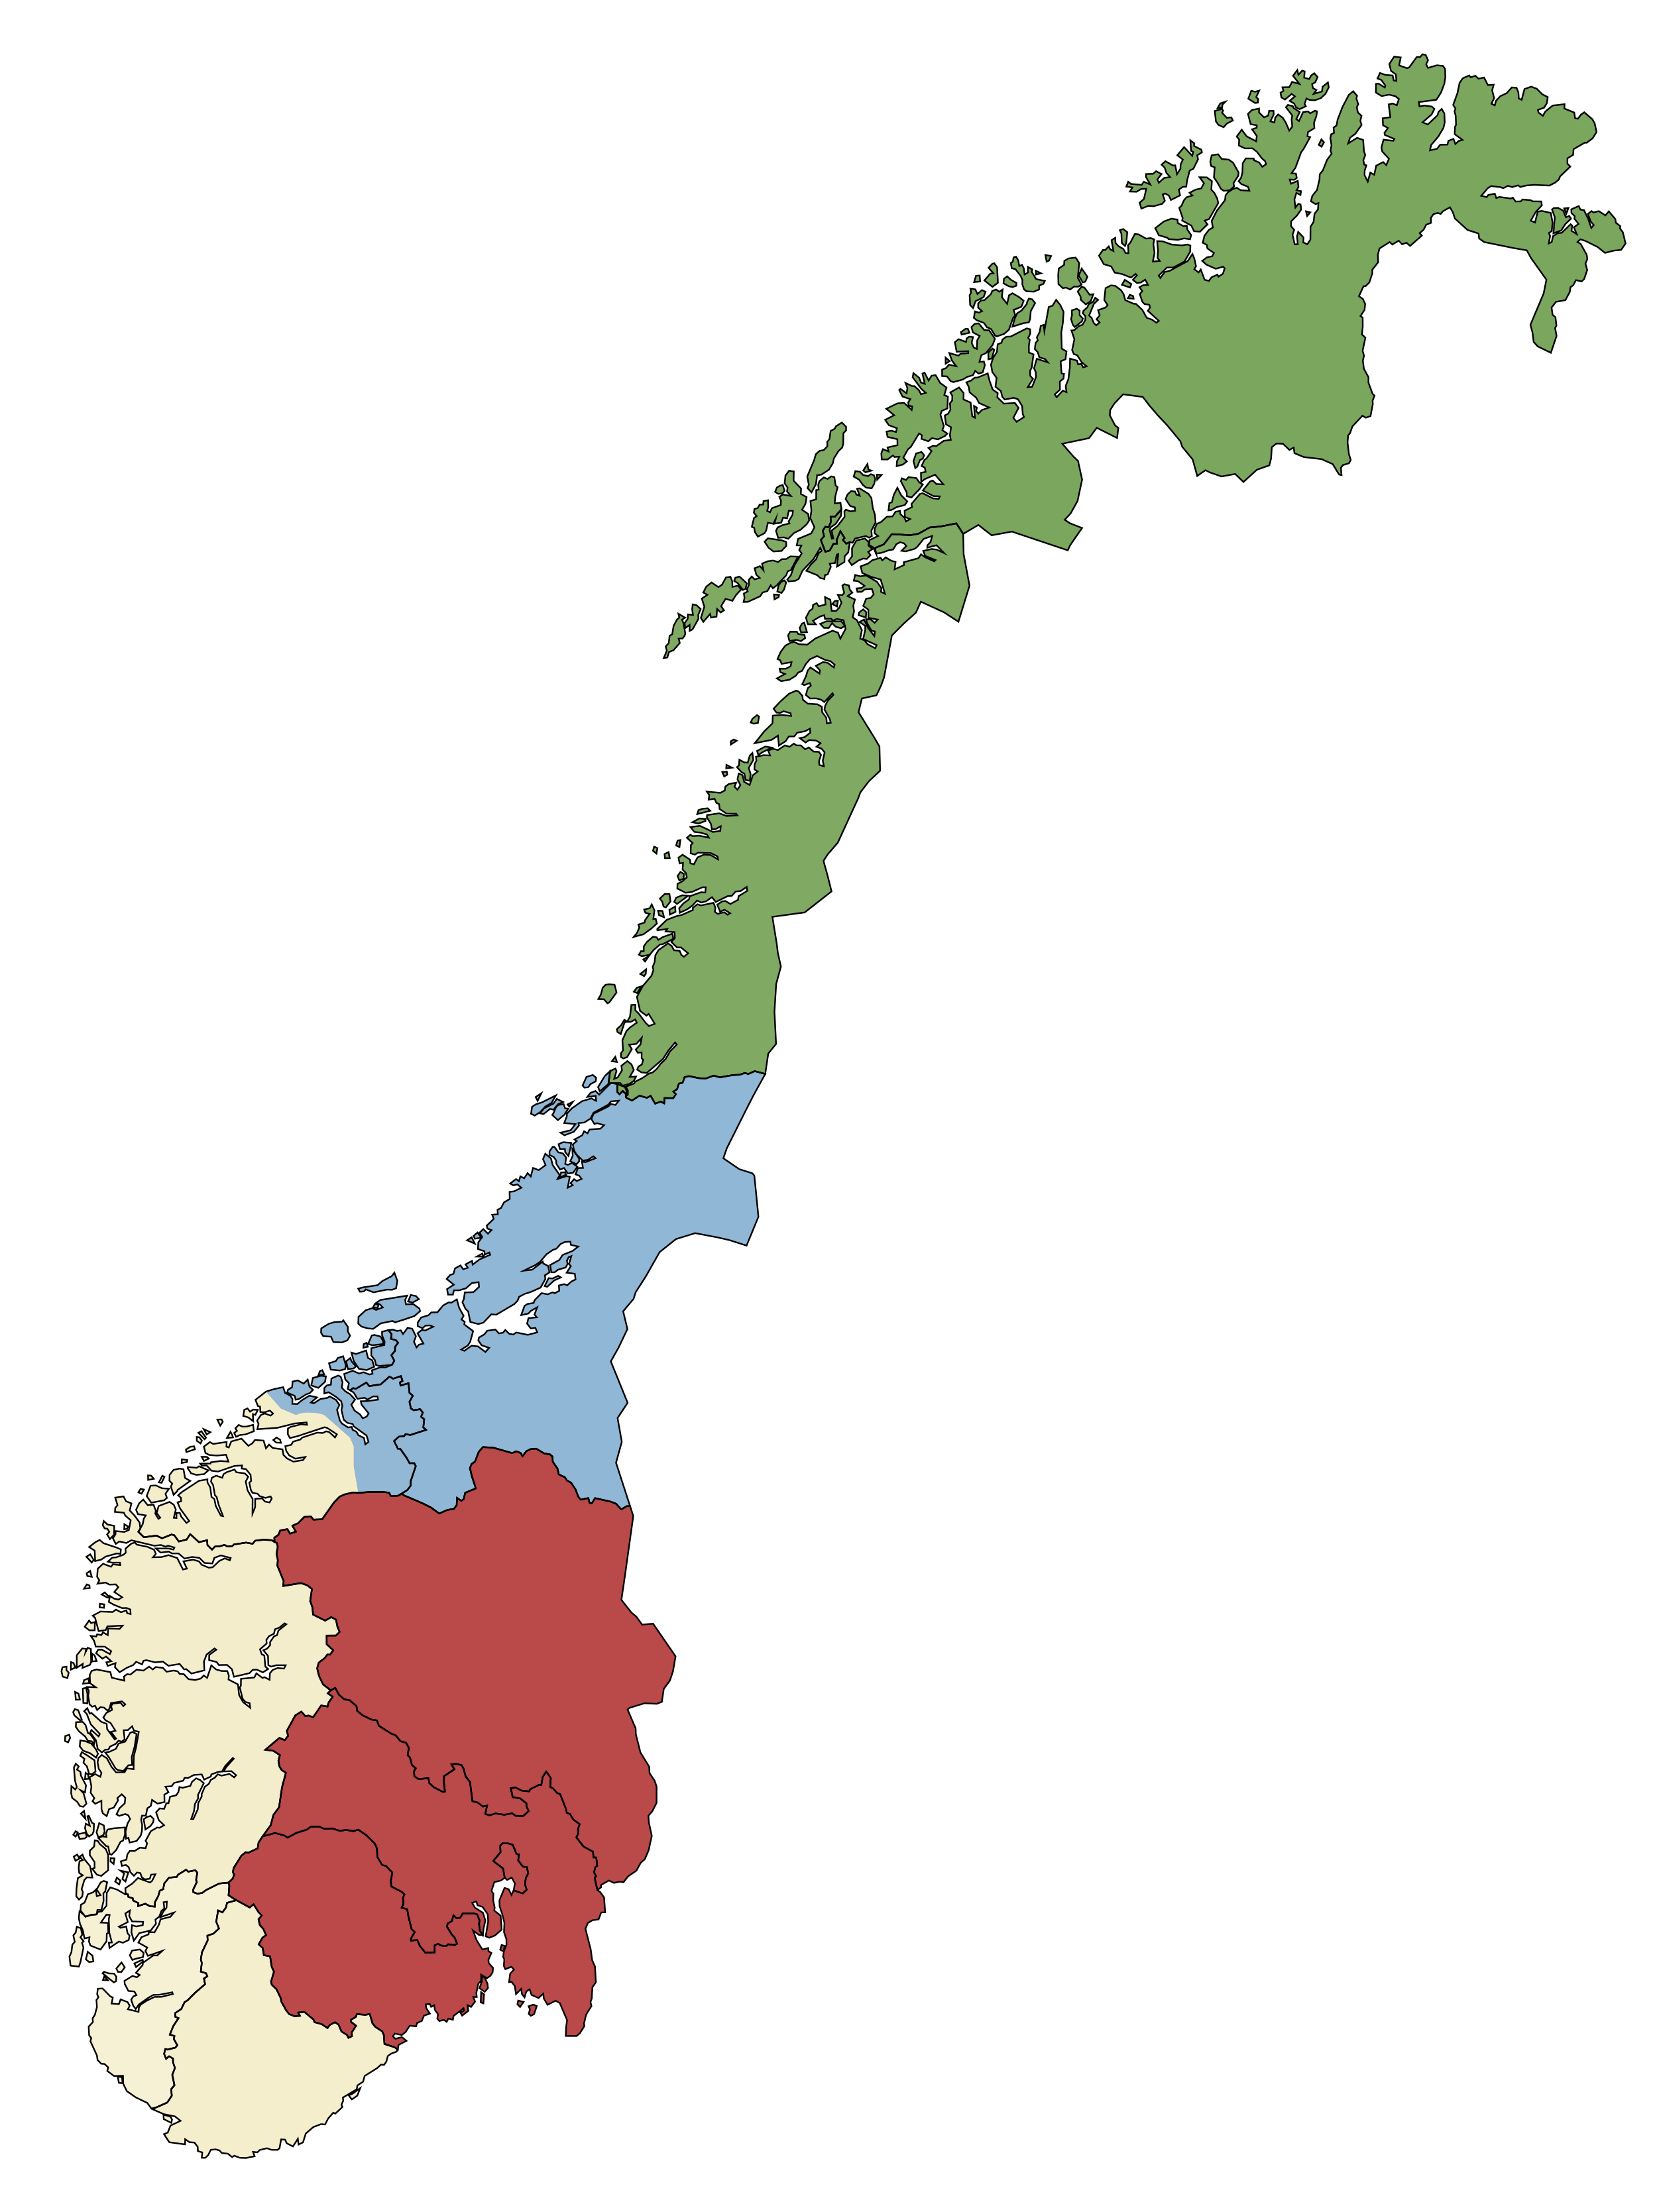
\includegraphics[width=\textwidth]{figures/3-dialects/fylke.png}};
        
    % % Temporary helper lines
    % \path[draw=red, line width=0.5mm] (0,-7) -- (0,7);
    % \path[draw=black] (1,-1)-- (1,7);
    % \path[draw=black] (2,-1)-- (2,7);
    % \path[draw=black] (3,1)-- (3,7);
    % \path[draw=black] (4,1)-- (4,7);
    % \path[draw=red] (5,3)-- (5,7);
    % \path[draw=black] (-1,-7) -- (-1,7);
    % \path[draw=black] (-2,-7) -- (-2,7);
    % \path[draw=black] (-3,-7) -- (-3,7);
    % \path[draw=black] (-4,-7) -- (-4,7);
    % \path[draw=red] (-5,-7) -- (-5,7);
    % \path[draw=red, line width=0.5mm] (-5,0)-- (5,0);
    % \path[draw=black] (-5,1)-- (3,1);
    % \path[draw=black] (-5,2)-- (3,2);
    % \path[draw=black] (-5,3)-- (3,3);
    % \path[draw=black] (-5,4)-- (5,4);
    % \path[draw=red] (-5,5)-- (5,5);
    % \path[draw=black] (-5,6)-- (5,6);
    % \path[draw=black] (-5,7)-- (5,7);
    % \path[draw=black] (-5,-1)-- (1,-1);
    % \path[draw=black] (-5,-2)-- (1,-2);
    % \path[draw=black] (-5,-3)-- (1,-3);
    % \path[draw=black] (-5,-4)-- (1,-4);
    % \path[draw=red] (-5,-5)-- (1,-5);
    % \path[draw=black] (-5,-6)-- (1,-6);
    % \path[draw=black] (-5,-7)-- (1,-7);
    
    % Informant locations:
    
    % North
    \node[loc = {}] (Hammerfest) at (2.85, 6.85) {};
    \node[loc = {}] (Kautokeino) at (3.0, 4.9) {};
    \node[loc = {}] (Kirkenes) at (5.5, 6.5) {};
    \node[loc = {}] (Kjoellefjord) at (4.1, 7.5) {};
    \node[loc = {}] (Lakselv) at (3.4, 6.3) {};
    \node[loc = {}] (Tana) at (4.6, 6.75) {};
    \node[loc = {}] (Vardoe) at (5.65, 7.2) {};
    \node[loc = {}] (Ballangen) at (0.5, 3.95) {};
    \node[loc = {}] (Beiarn) at (-0.4, 2.4) {};
    \node[loc = {}] (Bodoe) at (-0.5, 2.7) {};
    \node[loc = {}] (Hattfjelldal) at (-0.7, 0.9) {};
    \node[loc = {}] (HeroeyN) at (-1.4, 1.25) {};
    \node[loc = {}] (MoIRana) at (-0.55, 1.6) {};
    \node[loc = {}] (Myre) at (-0.3, 4.5) {};
    \node[loc = {}] (Narvik)  at (0.7, 4.0) {};
    \node[loc = {}] (Stamsund)  at (-0.7, 3.65) {};
    \node[loc = {}] (Steigen)  at (-0.25, 3.3) {};
    \node[loc = {}] (Soemna)  at (-1.45, 0.45) {};
    \node[loc = {}] (Botnhamn)  at (0.8, 5.3) {};
    \node[loc = {}] (Karlsoey)  at (1.5, 5.9) {};
    \node[loc = {}] (Kirkesdalen)  at (1.25, 4.7) {};
    \node[loc = {}] (Kvaefjord)  at (0.1, 4.3) {};
    \node[loc = {}] (Kvaenangen)  at (2.15, 5.95) {};
    \node[loc = {}] (Kaafjord)  at (2.77, 6.02) {};
    \node[loc = {}] (Lavangen)  at (0.8, 4.45) {};
    \node[loc = {}] (Medby)  at (0.4, 4.9) {};
    \node[loc = {}] (Medfjordvaer)  at (0.65, 5.25) {};
    \node[loc = {}] (Stonglandseidet)  at (0.55, 4.75) {};
    \node[loc = {}] (Tromsoe)  at (1.2, 5.5) {};
    
    % Troendersk
    \node[loc = {}] (Inderoey)  at (-2.05, -1.15) {};
    \node[loc = {}] (Lierne)  at (-0.75, -0.6) {};
    \node[loc = {}] (Meraaker)  at (-1.7, -1.65) {};
    \node[loc = {}] (Namdalen)  at (-1.4, -0.4) {};
    \node[loc = {}] (Bjugn)  at (-2.65, -1.3) {};
    \node[loc = {}] (Gauldal)  at (-2.1, -2.15) {};
    \node[loc = {}] (Oppdal)  at (-2.8, -2.6) {};
    \node[loc = {}] (Roeros)  at (-1.88, -2.65) {};
    \node[loc = {}] (Selbu)  at (-2.1, -1.88) {};
    \node[loc = {}] (Skaugdalen)  at (-2.5, -1.4) {};
    \node[loc = {}] (Stokkoeya)  at (-2.55, -0.95) {};
    \node[loc = {}] (Trondheim)  at (-2.4, -1.65) {};
    \node[loc = {}] (Aure)  at (-3.3, -1.75) {};
    \node[loc = {}] (Surnadal)  at (-3.2, -2.12) {};
    \node[loc = {}] (Todalen)  at (-3.3, -2.3) {};
    
    % West
    \node[loc = {}] (Bergen)  at (-5.3, -4.85) {};
    \node[loc = {}] (Boemlo)  at (-5.45, -5.55) {};
    \node[loc = {}] (Eidfjord)  at (-4.4, -4.95) {};
    \node[loc = {}] (Fusa)  at (-5.15, -5.15) {};
    \node[loc = {}] (Kvinnherad)  at (-4.95, -5.35) {};
    \node[loc = {}] (Lindaas)  at (-5.35, -4.5) {};
    \node[loc = {}] (Voss)  at (-4.7, -4.65) {};
    \node[loc = {}] (Bud)  at (-4.2, -2.15) {};
    \node[loc = {}] (HeroeyMR)  at (-4.9, -2.8) {};
    \node[loc = {}] (Rauma)  at (-3.88, -2.55) {};
    \node[loc = {}] (Stranda)  at (-4.28, -2.77) {};
    \node[loc = {}] (Volda)  at (-4.72, -2.95) {};
    \node[loc = {}] (Gjesdal)  at (-5.2, -6.68) {};
    \node[loc = {}] (Hjelmeland)  at (-5, -6.25) {};
    \node[loc = {}] (Karmoey)  at (-5.45, -6.1) {};
    \node[loc = {}] (Sokndal)  at (-4.95, -7.22) {};
    \node[loc = {}] (Stavanger)  at (-5.25, -6.5) {};
    \node[loc = {}] (Suldal)  at (-4.9, -6) {};
    \node[loc = {}] (Time)  at (-5.25, -6.8) {};
    \node[loc = {}] (Hyllestad)  at (-5.25, -4) {};
    \node[loc = {}] (Joelster)  at (-4.5, -3.65) {};
    \node[loc = {}] (Kalvaag)  at (-5.35, -3.3) {};
    \node[loc = {}] (Luster)  at (-4.05, -3.85) {};
    \node[loc = {}] (Stryn)  at (-4.45, -3.3) {};
    \node[loc = {}] (Evje)  at (-4.15, -7.1) {};
    \node[loc = {}] (Landvik)  at (-3.7, -7.4) {};
    \node[loc = {}] (Valle)  at (-4.23, -6.35) {};
    \node[loc = {}] (Vegaarshei)  at (-3.45, -6.9) {};
    \node[loc = {}] (Kristiansand)  at (-4.0, -7.55) {};
    \node[loc = {}] (Lyngdal)  at (-4.55, -7.55) {};
    \node[loc = {}] (Sirdal)  at (-4.7, -6.92) {};
    \node[loc = {}] (Vennesla)  at (-4.0, -7.4) {};
    \node[loc = {}] (Aaseral)  at (-4.4, -6.95) {};
    
    % East
    \node[loc = {}] (Enebakk)  at (-2.05, -5.78) {};
    \node[loc = {}] (Lommedalen)  at (-2.43, -5.6) {};
    \node[loc = {}] (Nes)  at (-1.95, -5.4) {};
    \node[loc = {}] (Darbu)  at (-2.88, -5.89) {};
    \node[loc = {}] (Flaa)  at (-3.0, -5.03) {};
    \node[loc = {}] (Rollag)  at (-3.13, -5.53) {};
    \node[loc = {}] (Sylling)  at (-2.58, -5.65) {};
    \node[loc = {}] (Aal)  at (-3.5, -4.7) {};
    \node[loc = {}] (Alvdal)  at (-2.3, -3.12) {};
    \node[loc = {}] (Dalsbygda)  at (-2.04, -2.69) {};
    \node[loc = {}] (Drevsjoe)  at (-1.56, -3.47) {};
    \node[loc = {}] (Kirkenaer)  at (-1.55, -5.04) {};
    \node[loc = {}] (Rena)  at (-1.98, -4.3) {};
    \node[loc = {}] (Stange)  at (-2.02, -4.73) {};
    \node[loc = {}] (Trysil)  at (-1.4, -4.0) {};
    \node[loc = {}] (Brekkom)  at (-2.63, -3.9) {};
    \node[loc = {}] (Gausdal)  at (-2.7, -4.0) {};
    \node[loc = {}] (Jevnaker)  at (-2.5, -5.2) {};
    \node[loc = {}] (Kvam)  at (-2.75, -3.58) {};
    \node[loc = {}] (Lom)  at (-3.5, -3.4) {};
    \node[loc = {}] (Gausdal)  at (-2.7, -4.0) {};
    \node[loc = {}] (Skreia)  at (-2.2, -4.82) {};
    \node[loc = {}] (Stange)  at (-2.02, -4.73) {};
    \node[loc = {}] (Vang)  at (-3.5, -4.18) {};
    \node[loc = {}] (Vestre Slidre)  at (-3.4, -4.2) {};
    \node[loc = {}] (Hjartdal)  at (-3.55, -5.9) {};
    \node[loc = {}] (Langesund)  at (-2.96, -6.62) {};
    \node[loc = {}] (Nissedal)  at (-3.65, -6.45) {};
    \node[loc = {}] (Tinn)  at (-3.4, -5.48) {};
    \node[loc = {}] (Vonje)  at (-4.03, -5.86) {};
    \node[loc = {}] (Brunlanes)  at (-2.9, -6.64) {};
    \node[loc = {}] (Hof)  at (-2.7, -6.05) {};
    \node[loc = {}] (Lardal)  at (-2.78, -6.15) {};
    \node[loc = {}] (Aremark)  at (-1.82, -6.36) {};
    \node[loc = {}] (Fredrikstad)  at (-2.2, -6.4) {};
    \node[loc = {}] (Roemskog)  at (-1.74, -5.83) {};
    
\begin{customlegend}[
    legend entries={
        North Norwegian,
        Tr\o{}nder,
        West Norwegian,
        East Norwegian,
        County borders,
        Informant locations
        },
    legend style={
        at={(5, -2)},
        nodes={inner xsep=4pt}
        },
    legend cell align={left},
]
    \addlegendimage{area legend,fill=mygreen}
    \addlegendimage{area legend,fill=myblue}
    \addlegendimage{area legend,fill=myyellow}
    \addlegendimage{area legend,fill=myred}
    \addlegendimage{no markers,line width=0.25mm}
    \addlegendimage{only marks,mark=*,red}
\end{customlegend}
\end{tikzpicture}

\end{document}
